\documentclass[11pt, oneside]{article}   	% use "amsart" instead of "article" for AMSLaTeX format
\usepackage{geometry}                		% See geometry.pdf to learn the layout options. There are lots.
\geometry{letterpaper}                   		% ... or a4paper or a5paper or ... 
%\geometry{landscape}                		% Activate for for rotated page geometry
%\usepackage[parfill]{parskip}    		% Activate to begin paragraphs with an empty line rather than an indent
\usepackage{graphicx}				% Use pdf, png, jpg, or eps� with pdflatex; use eps in DVI mode
								% TeX will automatically convert eps --> pdf in pdflatex		
\usepackage{amssymb}
\usepackage{amsmath}
\usepackage{parskip}
\usepackage{color}
\usepackage{hyperref}

\title{Using Cauchy}
%\author{The Author}
%\section{}
%\subsection*{}
\date{}							% Activate to display a given date or no date

\graphicspath{{/Users/telliott_admin/Dropbox/Tex/png/}}
% \begin{center} 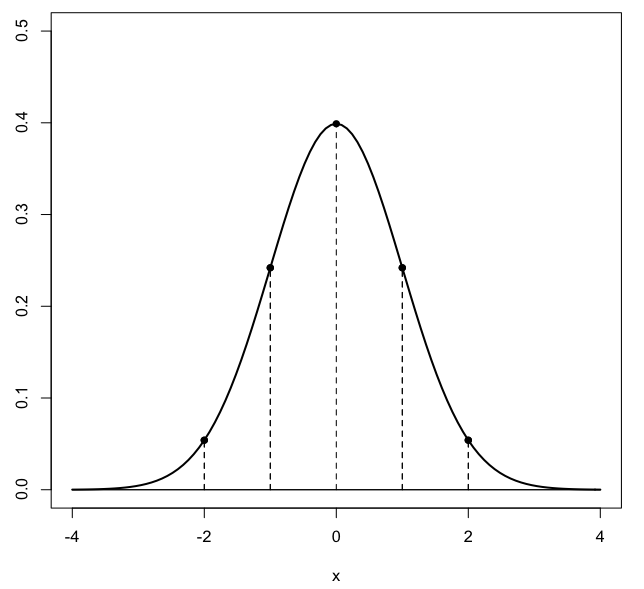
\includegraphics [scale=0.4] {gauss3.png} \end{center}
\begin{document}
\maketitle
\Large
In previous sections we derived three important theorems about complex functions.  (1) The Cauchy-Riemann equations (CRE) apply to analytic functions---functions that have derivatives---and vice-versa.
\[ u_x = v_y \]
\[ u_y = - v_x \]
We allow analytic functions to have a finite number of isolated singularities or poles where the function may "blow up."

(2) We used the CRE and Green's theorem to show that if a function is analytic everywhere in a simply-connected region, then the integral around any closed path in the region is zero.
\[ \oint f(z) \ dz = 0 \]
(3) On the other hand, if the region contains a singularity or pole, then we used a trick to show that the integral around \emph{any} closed path surrounding the pole has the same value.  This allows us to shrink the curve down to the immediate neighborhood of the pole and leads to the result in the limit as $z \rightarrow z_0$:
\[ \oint_C \frac{f(z)}{z - z_0} \ dz = 2 \pi i f(z_0) \]
(4) We can extend this result to a finite number of poles.  The value of the integral around all of them is the sum of the values for the individual poles.

\subsection*{Example 1}
Consider
\[ \oint \frac{6}{z(z-3)} \ dz \]
As shown in the figure, we are supposed to take for the curve $C$ the set of points $|z-3| = 5$, which is a circle of radius $5$ surrounding the point $z=3+0i$.
\begin{center} 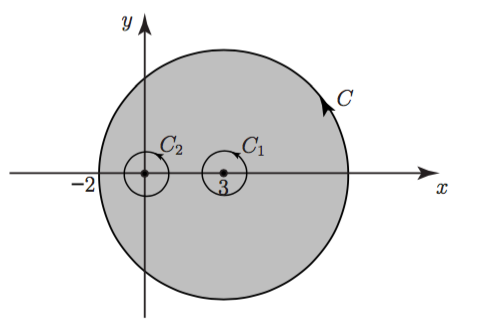
\includegraphics [scale=0.5] {cauchy2-fig1.png} \end{center}
This function does have two points of singularity, namely $z=0$ and $z=3$, so we expect that the value of the integral will not be zero.  We use (4) above to write
\[ \oint_C f(z) \ dz = \oint_{C_1} f(z) \ dz + \oint_{C_2} f(z) \ dz \]
We do not need to specify the curves because we will use (3) to calculate the values.

However, we do need to manipulate the function a bit.  We use the method of partial fractions.  Leaving aside the factor of $6$ for a moment:
\[ \frac{1}{z(z-3)} = \frac{A}{z} + \frac{B}{z-3} = \frac{A(z-3) + B(z)}{z(z-3)} \]
From looking at the numerator on the left- and right-hand sides, we see that $A = -B$ (because $Az + Bz = 0$), and that $-3A = 1$.  Hence
\[ A = -\frac{1}{3}, \ \ \ B = \frac{1}{3} \]
Recall the factor of $6$ and substitute for $A$ and $B$ in the middle expression to obtain:
\[ f(z) = \frac{-2}{z} + \frac{2}{z-3} \]
So now we can split the integrals for each curve into two parts.  We have:
\[ \oint_{C_1} f(z) \ dz + \oint_{C_2} f(z) \ dz \]
\[ = \oint_{C_1} \frac{-2}{z} \ dz + \oint_{C_1} \frac{2}{z-3} \ dz + \oint_{C_2} \frac{-2}{z} \ dz + \oint_{C_2} \frac{2}{z-3} \ dz  \]
Two of these four parts do not contain poles (the first and last), so these parts are just zero, and we have
\[ = \oint_{C_1} \frac{2}{z-3} \ dz + \oint_{C_2} \frac{-2}{z} \ dz  \]
At this point we can use (3) from above, that
\[ \oint_C \frac{f(z)}{z - z_0} \ dz = 2 \pi i f(z_0) \]
(recognizing that the denominator for the second integral can be written as $z - 0$).  So the result is $2 \pi i f(z_0)$ for both integrals, but the value of the function is just $2$ for the first term and $-2$ for the second term, which cancel.  In this case, the total integral is just zero.
Notice that the cancellation comes because $A = -B$, which we would obtain for any two factors $z$ and $z - a$ ($a \ne 0$).
\subsection*{Example 2}
Consider
\[ \oint \frac{z}{z^2 + 1} \ dz \]
This function has poles at $z = \pm i$.
\begin{center} 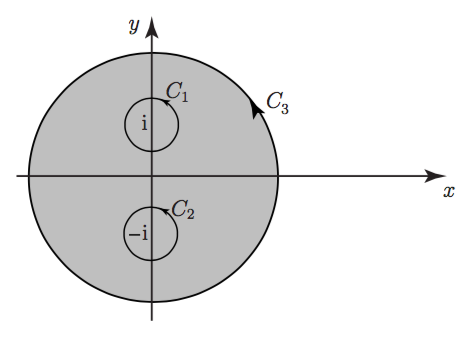
\includegraphics [scale=0.5] {cauchy2-fig2.png} \end{center}
We could see the poles by solving $z^2 + 1 = 0$ or we could factor
\[ z^2 + 1 = (z + i)(z - i) \]
This leads us to the idea of factoring as before
\[ \frac{z}{z^2 + 1} = \frac{A}{z+i} + \frac{B}{z-i} \]
By inspection, $A = B = 1/2$ is a solution, so
\[ \oint \frac{z}{z^2 + 1} \ dz = \oint \frac{1}{2(z+i)} + \frac{1}{2(z-i)} \ dz  \]
As before, curve $C_1$ encloses a pole only for the second term, and $C_2$ for the first term.  We use
\[ \oint_C \frac{f(z)}{z - z_0} \ dz = 2 \pi i f(z_0) \]
where the function is simply the value $1/2$.  So we obtain
\[ 2 \pi i \  \frac{1}{2} + 2 \pi i \ \frac{1}{2} = 2 \pi i \]

\end{document}  
